\documentclass{article}
\usepackage[left=2cm, right=2cm, top=3cm, bottom=3cm]{geometry}
\usepackage[utf8]{inputenc}
\usepackage{amsmath}
\usepackage{amsthm}
\usepackage{amssymb}
\usepackage{hyperref}
\usepackage{graphicx}
\usepackage{xcolor}

\hypersetup{
    colorlinks,
    citecolor=black,
    filecolor=black,
    linkcolor=black,
    urlcolor=black
}

\newcommand{\R}{\mathbb{R}}
\newcommand{\Rext}{\widetilde{\mathbb{R}}}
\newcommand{\DeltaEp}{\delta_{\varepsilon}}

\newenvironment{mytheorem}[1]
{\begin{theorem}[#1]\setlength{\leftskip}{2cm}}
{\end{theorem}}

\title{Teoria Analisi 1}

\begin{document}
\maketitle
\tableofcontents\newpage

\begin{flushleft}

\section{Teorema del differenziale (Lagrange - Rolle generalizzato) - Solo enunciato}
{2.2em}$f: I \subset \R, I$ intervallo, $x_0 \in I$, $x_0$ interno ad $I$, $f$ derivabile in $x_0$.
\\Allora: $\exists$ w: I $\rightarrow \R$ t.c. w è continua in $x_0$, w($x_0$) = 0 e
\[
    f(x_0) + f'(x_0)(x-x_0)+w(x)(x-x_0)
\]
\\dove: $f(x_0) + f'(x_0)(x-x_0)$ è la tangente
\\\hspace{2.3em} $w(x)(x-x_0)$ è l'errore causato da alcuni fattori, \underline{lo possiamo trascurare.}


\section{Teorema dell'unicità del limite}
\subsection{Enunciato}
$f: A \subset \R \rightarrow \R$, $x_0 \in \Rext$ punto di accumulazione per $A$
Se:
\begin{enumerate}
    \item $\lim_{x \to x_0} f(x) = l_1 \in \Rext$
    \item $\lim_{x \to x_0} f(x) = l_2 \in \Rext$
\end{enumerate}
Allora: $\mathbf{l_1 = l_2}$

\subsection{Dimostrazione}

\begin{enumerate}
    \item[ip1)] $\forall V l_1 $ intorno di $l_1 \exists U x_0$ intorno di $x_0$ t.c. $f(x)\in\forall l_1 $ per ogni $x\in (U x_0 \bigcap A) - \{0\}$
    \item[ip2)] $\forall V l_2 $ intorno di $l_2 \exists U' x_0$ intorno di $x_0$ t.c. $f(x)\in\forall l_2 $ per ogni $x\in (U' x_0 \bigcap A) - \{0\}$
\end{enumerate}

\begin{figure}[h]
    \centering
    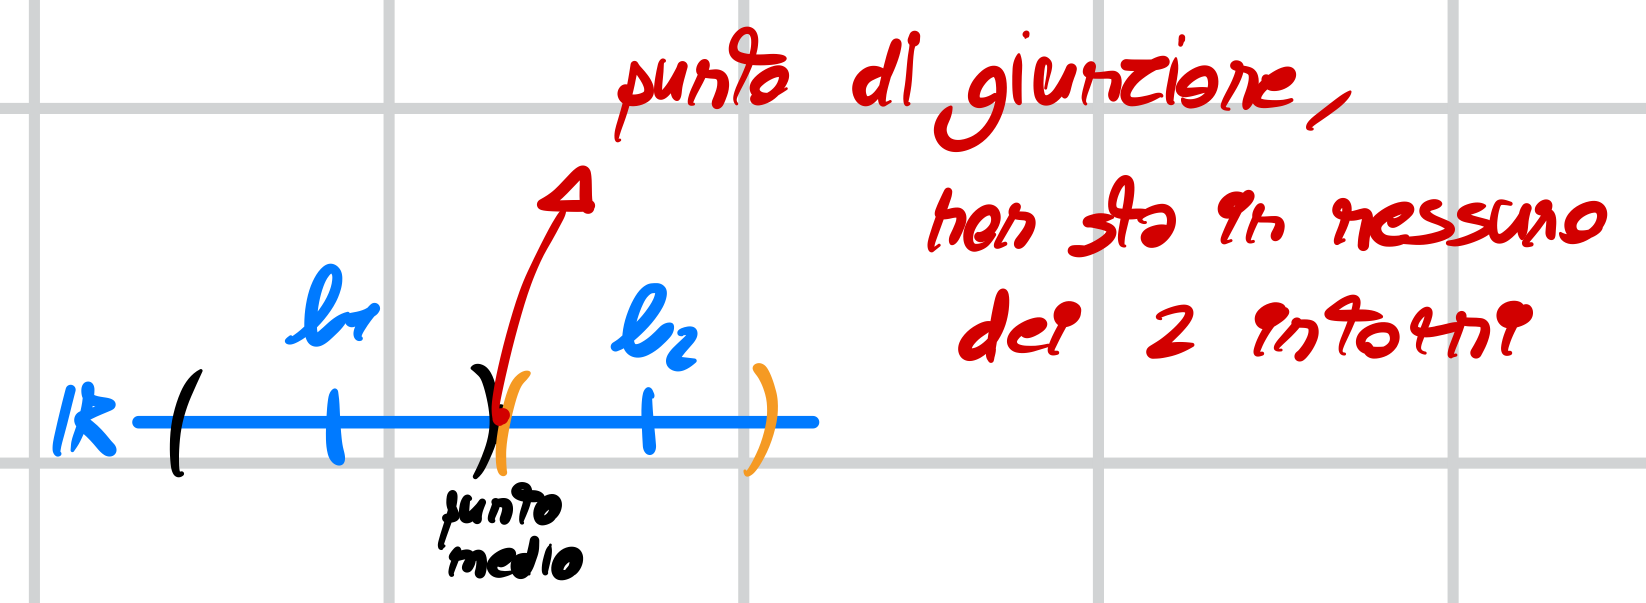
\includegraphics[width=10em]{./images/unicitaLimite.PNG}
\end{figure}

Per contraddizione: $l_1 \neq l_2$
\\Allora $\exists Vl_1, Vl_2$ intorni di $l_1$ e $l_2$ (rispettivamente) tali che: $Vl_1 \bigcup Vl_2 \neq \emptyset$
\\$Wx_0 = \bigcup U'x_0$ è un intorno di $x_0$
\\Sia $x \in(Wx_0 \bigcup A) - \{x_0\} \neq \emptyset$ (perché $x_0$ è di accumulazione)
\[
    \Rightarrow
    \begin{cases}
        f(x) \in Vl_1 \text{  (Per definizione di limite 1)}\\
        f(x) \in Vl_2 \text{  (Per definizione di limite 2)}
    \end{cases}
\]
\[
    \Rightarrow f(x) \in Vl_1 \bigcap Vl_2 \neq \emptyset \Rightarrow \mathbf{l_1 = l_2}. \mathbf{\textbf{ \underline{Contraddizione}}}
\]

\section{Teorema fondamentale del calcolo integrale (TFCI)}
\subsection{Enunciato}
$[a,b] \subset \R$, $a < b$. $f$ R-integrale su $[a,b]$.
\\$\exists x_1 \in [a,b]$ t.c. $f$ sia continua in $x_1$.
\\Fissato $x_0 \in $[a,b] e presa $F(x) = \int_{x_0}^{x}f(t)dt$, si ha che $F$ è derivabile in $x_1$ e $F'(x_1)=f(x_1)$
\subsection{Dimostrazione}
\[ 0 \leq \left| \frac{F(x) - F(x_1)}{x - x_1} - f(x_1) \right|, \quad x \neq x_1 \]
\[ = \left| \frac{\int_{x_0}^{x}f(t)dt-\int_{x_0}^{x_1}f(t)dt}{x - x_1} - f(x_1) \right|\]


\textbf{Dim:}

\begin{align*}
    0 &\leq \left| \frac{F(x) - F(x_1)}{x - x_1} - f(x_1) \right|, \quad x \neq x_1 \\
    &= \left| \frac{\int_{x_1}^{x} f(t) dt - \int_{x_1}^{x_1} f(t) dt}{x - x_1} - f(x_1) \right| \\
    &= \left| \frac{\int_{x_1}^{x} f(t) dt + \int_{x_1}^{x_1} f(t) dt - \int_{x_1}^{x_1} f(t) dt}{x - x_1} - f(x_1) \right| \\
    &= \left| \frac{\int_{x_1}^{x} f(t) dt - f(x_1)(x - x_1)}{x - x_1} \right| \\
    &= \left| \frac{\int_{x_1}^{x} (f(t) - \textcolor{red}{f(x_1)}) dt}{x - x_1} \right| \\
    &\textcolor{orange}{\leq} \frac{1}{x - x_1} \int_{x_1}^{x} |f(t) - f(x_1)| dt
\end{align*}
\textcolor{orange}{Dove abbiamo usato la \textbf{disuguaglianza integrale}.}\\
\textcolor{red}{\textbf{Nota:} Nel passaggio evidenziato in giallo, $c$ è una costante.}
\vspace{1em}
\\Ma $f$ è continua in $x_1 \iff $
\[\forall\epsilon>0\text{ }\exists \DeltaEp>0\text{ t.c. }\left|f(t) - f(x_1)\right|<\epsilon\text{ }\forall t / 0 < \left|t-x_1\right|<\DeltaEp\text{ }t\in[a,b]\]
Osservo che $t\in[x_1, x]$ (oppure $t\in[x, x_1]$, dipende come abbiamo disposto $x$ e $x_1$)
\\Implica che $\left|t-x_1\right| \leq \left|x - x_1\right|$
\\Sia allora $x\in[a, b] / \left|x-x_1\right|<\DeltaEp$. \underline{Con questo forziamo le due varibli a stare vicine fra loro}
\\Quindi $\left|t-x_1\right| \leq \left|x-x_1\right|<\DeltaEp$ e $\left|f(t) - f(x_1)\right|<\epsilon$
\\Allora $0\leq\left|\frac{F(x)-F(x_1)}{x-x_1}-f(x_1)\right| < \frac{1}{\left|x-x_1\right|}\left|\int_{x_1}^{x}\epsilon dt\right| = \epsilon \frac{\left|x-x_1\right|}{\left|x-x_1\right|} = \epsilon$
\\Ossia: $\forall \epsilon > 0$ $\exists \DeltaEp > 0$ t.c. $\left|\frac{F(x)-F(x_1)}{x-x_1}-f(x_1)\right|<\epsilon$ $\forall x$ t.c. $0<\left|x-x_1\right|<\DeltaEp$, $x\in[a,b]$
\\Cioè:$\lim_{x_1}\frac{F(x)-F(x_1)}{x-x_1}$ esiste e vale $f(x_1)$.
\\\centering \textbf{Quindi: $\mathbf{F'(x_1) = f(x_1)}$}



\end{flushleft}
\end{document}